%----------------------------------------------------------------------
\begin{frame}[c]{Where are we? The big picture}

\begin{itemize}
\item Algorithm Selection
  \begin{itemize}
    \item Portfolios
    \item Algorithm selection (for runtime)
  \end{itemize}
  \item Design decisions:\\ Local Search + Evo. Algorithms + Machine Learning 
  \item Empirical evaluation
  \item AAD for ML
  \begin{itemize}
    \item Hyperparameter optimization and Bayesian optimization 
    \item Neural architecture search (lecture given by Prof. Hutter)
  \end{itemize}
  \item[$\to$] Algorithm configuration 
  \begin{itemize}
    \item Basics 
    \item[$\to$] State of the art 
    \item Best practices 
  \end{itemize}
  \item Combinations of algorithm selection and configurations
  \item Algorithm control 
  \item Algorithm analysis 
  \item Project announcement and questions for exam 
\end{itemize}


\end{frame}
%-----------------------------------------------------------------------

%----------------------------------------------------------------------
\begin{frame}[c]{Preview: Learning Goals}

After this lecture, you should be able to \ldots
\begin{itemize}
  \item explain the ideas behind state-of-the-art algorithm configuration procedures
  \begin{itemize}
    \item SMAC: Bayesian Optimization (RF + EI) + Racing
    \item GGA: Gender-Based Genetic Algorithm for Algorithm Configuration
	\begin{itemize}
	  \item Competitive and non-competitive populations
	  \item Model-based GGA++
	  \item Genetic Engineering
	  \item Random Forests for Optimization Forecasting
	  \item Sexual Selection
	\end{itemize}
	\item iRace: Iterative Racing
    \begin{itemize}
      \item Sampling of new configurations
    \end{itemize}
  \end{itemize}  

\end{itemize}

\end{frame}
%----------------------------------------------------------------------

%%%%%%%%%%%%%%%%%%%%%%%%%%%%%%%%%%%%%%%%%%%%%%%%%%%%%%%%%%%%%%%%%%%%%%%%
\section{SMAC}
%%%%%%%%%%%%%%%%%%%%%%%%%%%%%%%%%%%%%%%%%%%%%%%%%%%%%%%%%%%%%%%%%%%%%%%%

%-------------------------------------------------------------
\begin{frame}
\frametitle{SMAC in a Nutshell} \vspace*{-1mm}

Combine Bayesian optimization with aggressive racing\\
~~~~~~~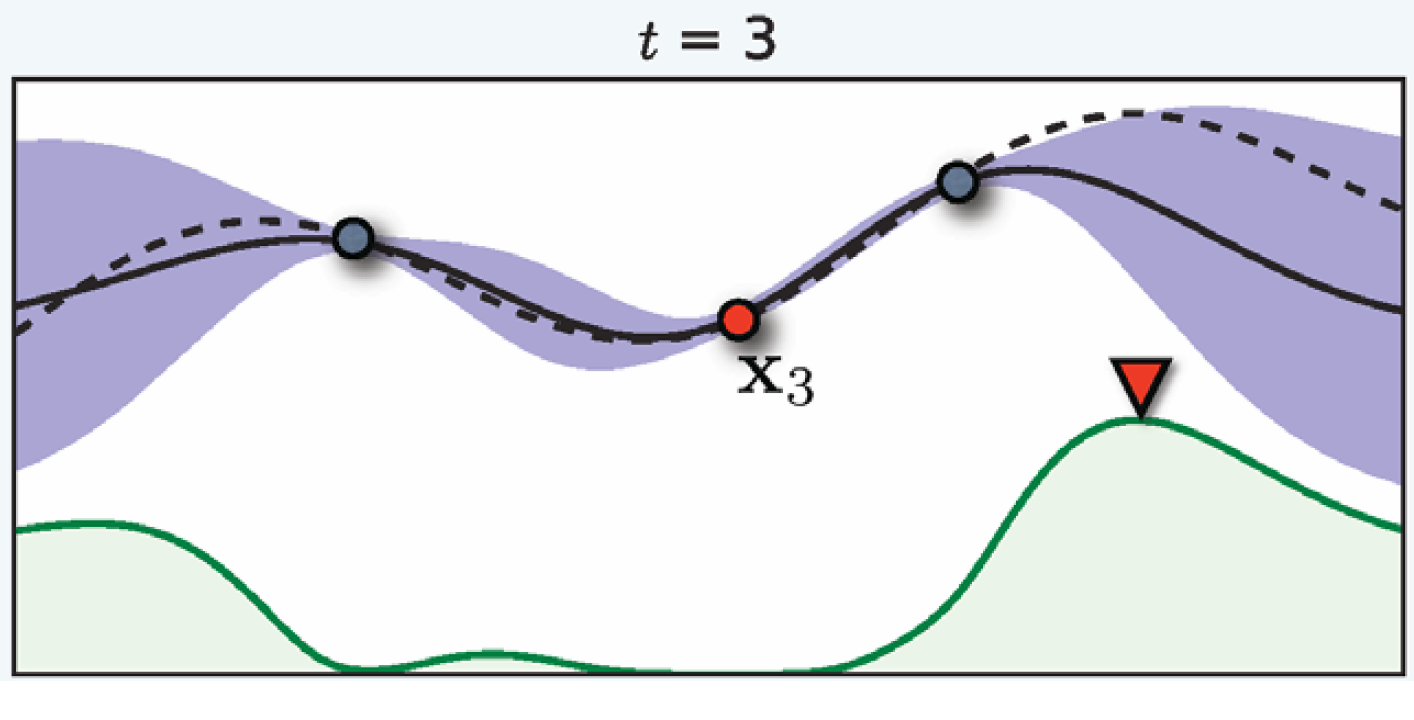
\includegraphics[width=0.5\textwidth]{images/my_lecture12/bo_pic2.png}\\

One SMAC iteration:
\begin{itemize}
	\item Construct a model to predict performance
	\item Use that model to select promising configurations
	\item Compare each of the selected configurations against the best known 
	\begin{itemize}
		\item[-] \alert{Using a similar procedure as FocusedILS}
	\end{itemize}
\end{itemize}

\bigskip
\pause
The details are in SMAC's \alert{empirical performance model}

\end{frame}


%----------------------------------------------------------------------
\begin{frame}[c]{What are Empirical Performance Models?}

\begin{block}{Definition: Empirical Performance Models (EPMs)}
Empirical performance models map
\begin{itemize} 
  \item parameter configuration $\conf \in \pcs$ of an algorithm and 
  \item instance $\inst \in \insts$
\end{itemize}
to the cost $c(\conf,\inst)$ of $\conf$ applied to $\inst$:

\begin{equation}
\surro: \pcs \times \insts \to \perf \nonumber
\end{equation}
\end{block}

\pause
\begin{block}{Examples of Cost Metrics}
\begin{itemize}
  \item runtime
  \item success probability of an algorithm
  \item solution quality an optimization algorithm achieves in a fixed time
  \item error of machine learning algorithm
\end{itemize}
\end{block}

\end{frame}
%-----------------------------------------------------------------------
%----------------------------------------------------------------------
\begin{frame}[c]{Inputs of an EPM?}

\begin{block}{Instances Features}
\begin{itemize}
  \item cheap-to-compute numerical representations of instances
  \item have to reflect properties of the instance related to algorithm's performance
  \item[$\leadsto$] list of features: $\feat(\inst) = [f_1, \ldots, f_m]^\intercal$ 
  \item often quite redundant; use of PCA to reduce dimensionality
  \item (see lectures on algorithm selection for examples)
\end{itemize}
\end{block}

\pause

\begin{block}{Parameter Configuration}
\begin{itemize}
  \item Settings of all parameters
  \item Note: freely adjustable\\ $\leadsto$ some transformations cannot be applied to them (e.g., PCA)  
  \item[$\leadsto$] list of parameter values $\conf := [\conf_1, \ldots, \conf_k]$
  \item Domains of each parameter $\Theta_1, \ldots, \Theta_k$
\end{itemize}
\end{block}

\end{frame}
%-----------------------------------------------------------------------
%----------------------------------------------------------------------
\begin{frame}[c]{Empirical Performance Models (EPMs):\\Predictions in
Joint Space of Instances \& Configurations}

\begin{multicols}{2}
\begin{center}
\includegraphics[height=4cm]{images/lecture7/figures__default_matrix__2d__redone__SPEAR-ibm-swv-al-truematrix-testC_testI}\\
True performance
\end{center}
\columnbreak
\begin{center}
\includegraphics[height=4cm]{images/lecture7/figures__default_matrix__2d__redone__SPEAR-ibm-swv-al-RF-def-10000testC_testI}\\
Predicted performance
\end{center}
\end{multicols}

\begin{itemize}  
    \item 302\,000 runs: 1000 configurations for each of 302 instances  
    \item Darker entries are faster runs!
\end{itemize}

\end{frame}
%-----------------------------------------------------------------------


%----------------------------------------------------------------------
\begin{frame}[c]{How we use EPMs in SMAC}

\begin{itemize}
  \item We keep track of all algorithm runs we execute
  \item Each run uses a $\conf_i$ on an instance $\pi_i$ with features $z_{\pi_i}$ and yields cost $y_i=c(\conf_i,\inst_i)$
  \begin{itemize}
  	\item[-] This constitutes a data point $\langle{} (\conf_i, z_{\inst_i}), y_i \rangle$
  	\item[-] We use this data to learn an EPM $\hat{c}: \confs \times \mathcal{F} \rightarrow \mathds{R}$
  \end{itemize}
  
  \pause
  \bigskip
  
  \item Algorithm configuration aims to minimize \alert{$c(\conf) = \mathds{E}_{\inst \sim \instD} [c(\conf,\inst)]$}
  \item Our model predicts on a per-instance level 
  \item We thus aggregate predictions over instances from distribution $D$:
  \begin{itemize}
  	\item \alert{$\hat{c}(\conf) = \mathds{E}_{\pi \sim D} [\surro(\conf, \pi)]$}
  	\item Naive approach: predict for each instance and then average
  \end{itemize}
  
\end{itemize}

\end{frame}
%-----------------------------------------------------------------------

%----------------------------------------------------------------------
\begin{frame}[c]{Reminder: Random Forests}

Ensembles of decision trees or regression trees

Training for $N$ data points
\begin{itemize}
  	\item Draw $T$ \alert{bootstrap samples} of the data
  	\myit{
  		\item[-] I.e., $T$ times, draw $N$ data points with repetitions 
  	}
  	\item For each bootstrap sample, fit a \alert{randomized} regression tree
\end{itemize}
  
Prediction
\begin{itemize}
  	\item Predict with each of the T trees
  	\item Return \alert{empirical mean and variance} across these T predictions
\end{itemize}
\end{frame}
%-----------------------------------------------------------------------
% %----------------------------------------------------------------------
% \begin{frame}[c]{Fitting a Regression Tree}
% 
% \includegraphics[width=0.9\textwidth]{images/lecture12/RF_data.png}
% 
% \end{frame}
% %-----------------------------------------------------------------------
% %----------------------------------------------------------------------
% \begin{frame}[c]{Fitting a Regression Tree}
% 
% \myit{
% 	\item In each internal node: only store split criterion used
% 	\item In each leaf: store mean of runtimes
% }
% 
% \includegraphics[width=0.9\textwidth]{images/lecture12/RF_built.png}
% 
% \pause
% \vspace*{-4.5cm}
% \myit{
% 	\item What would be the tree's prediction for a new data point (param$_1$,feature$_2$,param$_3$) = (true, 4.7, red)$?
% 	\myit{
% 		\item[\voteblue{}] 3.7
% 		\item[\voteyellow{}] 1.65
% 	}
% }
% 
% \end{frame}
% %-----------------------------------------------------------------------


%-----------------------------------------------------------------------
\begin{frame}[c]{SMAC: Putting it all Together}
%\\\litw{Hutter et al. 2011}}

\LinesNotNumbered
\begin{algorithm}[H]
\Input{%
instance set $\insts$,
Algorithm $\algo$ with configuration space $\confs$,
Initial configuration $\conf_0$,
performance metric $c$,
Configuration budget $b$
}
\Output{best incumbent configuration $\hat{\conf}$}
\BlankLine
run history H $\leftarrow$ initial design based on $\conf_0$; \tcp*{H = $(\conf, \inst, c(\inst,\conf))_i$}
\While{$b$ remains} {
   	\pause
	$\epm \leftarrow$ train empirical performance model based on run history H;\\
	\pause
	$\confs_{challengers} \leftarrow$ select configurations based on $\epm$;\\
	\pause
	$\hat{\conf}$, H $\leftarrow$ intensify($\confs_{challengers}$, $\hat{\conf}$);
}
\pause
\Return{$\hat{\conf}$}
\caption{SMAC}
\end{algorithm}

\end{frame}
%-----------------------------------------------------------------------

%-----------------------------------------------------------------------
\begin{frame}[c, fragile]{Intensify for a Single Challenger}
\LinesNotNumbered

Similar to FocusedILS:

\bigskip

\begin{algorithm}[H]
\Input{%
challenger configurations $\conf$,
incumbent configuration $\hat{\conf}$
}
\Output{best incumbent configuration $\hat{\conf}$}
\BlankLine
new run with $\hat{\conf}$;\\
\pause
$N \leftarrow 1$;\\
\While{$\conf$ has less runs than $\hat{\conf}$} {
	\pause
	sample and run $N$ instances $\conf$ has not run on but $\hat{\conf}$ has;\\
	\pause
	\If {$\hat{\conf}$ better than $\conf$} 
	{
		\tcp{See ParamILS for ``better''}  
		\Return{$\hat{\conf}$
	}
}
$N \leftarrow 2 \cdot N$;\\
}
\pause
\Return{$\hat{\conf} \leftarrow \conf$}
\caption{Intensify (only for a \textbf{single challenger})}

\end{algorithm}

\medskip
\pause
SMAC also uses adaptive capping inside of \textit{intensify} 
for runtime scenarios 

\end{frame}
%-----------------------------------------------------------------------
%----------------------------------------------------------------------
\begin{frame}[c]{Reminder: Handling of Censored Data}

\begin{block}{Censored Data}
Because of adaptive capping:
\begin{itemize}
  \item Only lower bound of runtime is known 
  \item Censoring can be at different cutoffs 
\end{itemize}
\end{block}

\pause

\begin{algorithm}[H]
\Input{Uncensored data $\mathbf{X}_{\text{u}}, \mathbf{y}_{\text{u}}$, Censored data $\mathbf{X}_{\text{c}}, \mathbf{y}_{\text{c}}$}
\Output{Imputed values $y_{\text{imp}}$ for $\mathbf{X}_{\text{c}}$}
\BlankLine
EPM.fit($\mathbf{X}_{\text{u}}, \mathbf{y}_{\text{u}}$);\\
\While{not converged} {
	\ForEach{censored sample $i$} {
		$\mu,\sigma^2$ := EPM.predict($\mathbf{X}_{\text{c}}^{(i)}$);\\
		$\mathbf{y}_{\text{imp}}^{(i)}$ := mean of $\mathcal{N}(\mu, \sigma^2)_{\geq \mathbf{y}_{\text{c}}^{(i)}}$;\\
	}
	EPM.fit($\mathbf{X}_{\text{u}} || \mathbf{X}_{\text{c}}, \mathbf{y}_{\text{u}} || \mathbf{y}_{\text{imp}}$);\\
}
\Return{$\mathbf{y}_{\text{imp}}$}
\end{algorithm}

\end{frame}
%-----------------------------------------------------------------------


%%%%%%%%%%%%%%%%%%%%%%%%%%%%%%%%%%%%%%%%%%%%%%%%%%%%%%%%%%%%%%%%%%%%%%%%
\section{GGA}
%%%%%%%%%%%%%%%%%%%%%%%%%%%%%%%%%%%%%%%%%%%%%%%%%%%%%%%%%%%%%%%%%%%%%%%%

%----------------------------------------------------------------------
\begin{frame}[c]{GGA: Genetic Algorithm for AC}

\begin{block}{Recap: Genetic Algorithms}
\begin{center} 
	\includegraphics[width=0.75\textwidth]{images/ea.png}  
\end{center}
\end{block}

\end{frame}
%----------------------------------------------------------------------

%-----------------------------------------------------------------------
\begin{frame}[c]{GGA~\litw{C. Ansotegui et al, 2009}}

Genetic algorithm:
\begin{itemize}
  \item Population of individuals as genomes (i.e., solution candidates)
  \item Modify population by
  \begin{itemize}
    \item Mutations (i.e., random changes) 
    \item Crossover (i.e., combination of 2 parents to form an offspring )
  \end{itemize}
\end{itemize}

\medskip
\pause

Genetic algorithm for Algorithm Configuration
\begin{itemize}
  \item Genome = parameter configuration
  \item Crossover: Combine of 2 configurations to form a new configuration 
\end{itemize}

\medskip
\pause

Two genders in the population (competitive and non-competitive)
\begin{itemize}
  \item Selection pressure only on one gender
  \item Preserves diversity of the population 
\end{itemize}

\end{frame}
%-----------------------------------------------------------------------

%-----------------------------------------------------------------------
\begin{frame}[c]{GGA: Crossover Operator}

\centering
\includegraphics[width=0.7\textwidth]{images/gga_crossover}

{\footnotesize Source: \lit{C. Ansotegui et al, 2015}}

\medskip

N: non-competitive C: competitive

\end{frame}
%-----------------------------------------------------------------------

%-----------------------------------------------------------------------
\begin{frame}[c]{GGA: Racing and Capping}

Can exploit parallel resources
\begin{itemize}
  \item Evaluate population members in parallel
  \item Adaptive capping: can stop when the first k succeed  
\end{itemize}

\pause
\medskip

Use $N$ instances to evaluate configurations
\begin{itemize}
  \item Increase N in each generation
  \item Linear increase from $N_{\text{start}}$ to $N_{\text{end}}$
  \item Problem: user has to specify \#generations ahead of time
\end{itemize}

\end{frame}
%-----------------------------------------------------------------------


%-----------------------------------------------------------------------
\begin{frame}[c]{GGA++: Model-based GGA \litw{Ansotegui et al, 2015}}

\begin{itemize}
  \item How would you use an EPM in GGA? \hands
  \pause
  \item Idea: Guide evolution of population by EPM
  \begin{itemize}
    \item influences the balance between exploration and exploitation of GAs
    \item evolve some configurations with the help of the EPM\\
    	  and some others by the original crossover/mutation operators
  \end{itemize}
  \medskip
  \pause
  \item 3 new main ingredients:
  \begin{enumerate}
    \item Genetic Engineering
    \item Selection of non-competitive mating partners based on their attractiveness
    \item Building decision trees (that will form random forests) with a bias towards better predictive performance around function extrema
  \end{enumerate}
\end{itemize}

\end{frame}
%-----------------------------------------------------------------------

%-----------------------------------------------------------------------
\begin{frame}[c]{Genetic Engineering}

\begin{itemize}
  \item Setting: Two individuals want to produce offspring
  \item[$\leadsto$] Many different ways how two individuals can be combined
  \pause
  \item[$\leadsto$] EPM can guide the recombination
  \pause
  \item[$\leadsto$] Limited focused search in space spanned by the two parents
  \pause
  \medskip
  \item Approach:
  \begin{enumerate}
    \item For each tree in the forest, gather all leaves that any potential offspring of the two parents could fall into
    \pause
    \item For each leaf, randomly sample a number $k$ of full assignments to the parameters
    \pause
    \item Select offspring with best $\surro(\conf)$ using entire random forest
  \end{enumerate}
\end{itemize}

\end{frame}
%-----------------------------------------------------------------------
%-----------------------------------------------------------------------
\begin{frame}[c]{Random Forests for Optimization Forecasting}

\begin{itemize}
  \item SMAC's EPM should have a high accuracy everywhere in $\pcs$
  \item However for optimization, high-performance areas are more important 
  \pause
  \medskip
  \item Idea: Higher resolution splits in high-performance areas
  \pause
  \item Concrete: Try to separate the $10\%$ best configurations from the rest\\ in each each split
  \item[$\leadsto$] Better predictions in high-performance areas
\end{itemize}

\bigskip
\pause
Note: SMAC achieves a similar effect by training its EPM on $\log(y)$

\end{frame}
%-----------------------------------------------------------------------
%-----------------------------------------------------------------------
\begin{frame}[c]{Sexual Selection}

\begin{itemize}
  \item Recap: GGA has two populations
  \pause
  \item Idea: giving preference to mating with more attractive partners
  \pause
  \item The competitive individuals are already filtered
  \item[$\leadsto$] competitive individuals choose their partners from the non-competitive subpopulation
  \begin{itemize}
    \item probability proportional to the estimated fitness of the partner
    \item using an EPM
  \end{itemize}
  \pause
  \medskip
  \item Risk of too strong exploitation and too little exploration
  \begin{itemize}
    \item non-competitive subpopulation should ensure exploration (diversification)
    \item Sexual selection introduces competition in the  non-competitive subpopulation
    \item[$\leadsto$] Less diversification in the population
  \end{itemize}
\end{itemize}

\end{frame}
%-----------------------------------------------------------------------

%%%%%%%%%%%%%%%%%%%%%%%%%%%%%%%%%%%%%%%%%%%%%%%%%%%%%%%%%%%%%%%%%%%%%%%%
\section{iRace}
%%%%%%%%%%%%%%%%%%%%%%%%%%%%%%%%%%%%%%%%%%%%%%%%%%%%%%%%%%%%%%%%%%%%%%%%

%-----------------------------------------------------------------------
\begin{frame}[c]{F-race \litw{Birattari et al, 2002}}

\begin{itemize}
  \item Idea: Sample a set of configurations and race them
  \item Uses a statistical test to check whether $\conf$ is inferior
  \begin{itemize}
  	\item[-] Namely, the F-test (giving F-Race its name)
  \end{itemize}
\end{itemize}

\pause
\bigskip

Visualization of how many runs are performed for each configuration:
\begin{center}
\includegraphics[width=0.71\textwidth]{images/irace_racing}\\
\end{center}

\end{frame}
%-----------------------------------------------------------------------

%-----------------------------------------------------------------------
\begin{frame}[c,fragile]{Iterated F-race~\litw{L\'{o}pez-Ib\'{a}\~{n}ez et al, 2011, 2016}}

Basic idea:
\begin{itemize}
	\item Use F-Race as a building block
	\item Gather configurations to race via estimation of distribution algorithm
	\item Short name: iRace
\end{itemize}

\begin{center}
\includegraphics[width=0.71\textwidth]{images/irace_workflow}\\
\end{center}

\end{frame}
%-----------------------------------------------------------------------

%-----------------------------------------------------------------------
\begin{frame}[c,fragile]{iRace Magic}

iRace has many magic numbers/ design decisions

\begin{itemize}
  \item Number of iterations for a given budget
  \item Budget per race
  \item Number of configurations per race
  \item Statistical test to reject configurations
  \item How to sample new configurations
\end{itemize}

\end{frame}
%-----------------------------------------------------------------------

%-----------------------------------------------------------------------
\begin{frame}[c,fragile]{Irace: Number of iterations and budget}


Number of iterations:
\begin{equation}
N^{\text{iter}} = \lfloor 2 + \log{N^{\text{param}}} \rfloor \nonumber
\end{equation}

\medskip

\begin{itemize}
  \item at least $2$ iterations to allow for some intensification
  \item more iterations for more parameters
\end{itemize}

\bigskip
\pause

Budget:
\begin{equation}
B_j = \frac{B - B^{\text{used}}}{N^{\text{iter}}-j +1} \nonumber
\end{equation}

\begin{itemize}
  \item $\approx$ equally distributed budget
\end{itemize}

\end{frame}
%-----------------------------------------------------------------------
%-----------------------------------------------------------------------
\begin{frame}[c]{iRace: Number of Configurations per Race}

\begin{equation}
|\Theta_j| = N_j = \left\lfloor \frac{B_j}{T^{\text{first}} + T^{\text{each}} \cdot \min(5,j)} \right\rfloor \nonumber
\end{equation}

\begin{itemize}
  \item number of candidate configurations decreases with the number of iterations
  \item Constant after after the fifth race
  \item $T^{\text{first}}=5$ is the number of instances needed for the first test
\end{itemize}

\end{frame}
%-----------------------------------------------------------------------
%-----------------------------------------------------------------------
\begin{frame}[c]{iRace: Sampling of new Configurations (1)}

\begin{itemize}
  \item a new value is sampled for each parameter $\conf_d$
  \item each parameter has an associated distribution
  \item new configurations are sampled from parent distributions
\end{itemize}

\pause
\medskip

\begin{itemize}
  \item Parent configuration $\theta_z$ selected with probability: 
\end{itemize}

\begin{equation}
p_z = \frac{N^{\text{elite}}_{j-1} - r_z +1}{N^{\text{elite}}_{j-1} \cdot (N^{\text{elite}}_{j-1} + 1)  /2}\nonumber
\end{equation}

\begin{itemize}
  \item rank $r_z$ of $\theta_z$\\
  $\leadsto$ configurations with higher rank have higher probability
  \bigskip
  \item generated configurations inherit the probability distributions of their parents
  
\end{itemize}

\end{frame}
%-----------------------------------------------------------------------
%-----------------------------------------------------------------------
\begin{frame}[c]{iRace: Sampling of new Configurations (2): Numerical}

\begin{itemize}
  \item Value range $[\conf_{min}, \conf_{max} ]$
  \item sampling from truncated normal distribution $\mathcal{N}(\conf^z_d, (\sigma^j_d)^2)_{x_{min} \leq x \leq x_{max}}$ 
  \item default $\sigma^j_d = \frac{\conf_{max} - \conf_{min}}{2}$ and decreased in each iteration
\end{itemize}

\pause

\begin{equation}
\sigma^j_d = \sigma^{j-1}_d \cdot \left(\frac{1}{N^{\text{new}}_j}\right)^{1/N^{\text{param}}}\nonumber
\end{equation}

$\leadsto$ more exploitation in later iterations

\pause
\medskip

integer-parameters are rounded to nearest integer

\end{frame}
%-----------------------------------------------------------------------
%-----------------------------------------------------------------------
\begin{frame}[c]{iRace: Sampling of new Configurations (3): Categorical}

\begin{itemize}
  \item values: $\{x_1,x_2,\ldots,x_{n_d}\}$
  \item first iteration ($j=1$): uniformly at random
  \item following iterations, updated according to
\end{itemize}

\begin{equation}
P^{j,z}(\conf_d = x_j)  = P^{j-1,z}(\conf_d=x_j)\cdot \left(1 - \frac{j-1}{N^{\text{iter}}} \right) + \Delta P \nonumber
\end{equation}

where

\begin{equation}
\Delta P = \begin{cases}
  \frac{j-1}{N^{\text{iter}}}, 	& \text{if } x_j = x_z,\\
  0								& otherwise.
\end{cases}\nonumber
\end{equation}

\begin{itemize}
  \item[$\leadsto$] Probability of parent value increases
  \item[$\leadsto$] All other probabilities decrease
\end{itemize}

\end{frame}
%-----------------------------------------------------------------------



%-----------------------------------------------------------------------
\begin{frame}[c,fragile]{Iterated F-race~\litw{L\'{o}pez-Ib\'{a}\~{n}ez et al, 2011, 2016}}

Basic idea:
\begin{itemize}
	\item Use F-Race as a building block
	\item Gather configurations to race via estimation of distribution algorithm
\end{itemize}

\pause
\medskip
Advantages 
\begin{itemize}
	\item Can \alert{parallelize easily}: runs of each racing iteration are independent 
	\item Well-supported software package (for the community that uses R)
\end{itemize}

\pause
\medskip
(Out-dated) Disadvantages 
\begin{itemize}
	\item Does not support adaptive capping
	\begin{itemize}
		\item recently introduced \lit{Caceres et al. LION 2017}
	\end{itemize}
	\item The estimation of distribution component is not very strong for complex search spaces
	\begin{itemize}
		\item recently extended to use EPMs \lit{Caceres et al. GECCO 2017}
	\end{itemize}
\end{itemize}

\end{frame}
%-----------------------------------------------------------------------




%-----------------------------------------------------------------------
\begin{frame}{Empirical Comparison of Algorithm Configurators}

\begin{itemize}
	\item[] Experimental setup \lit{Hutter et al. LION 2011}
	\begin{itemize}
		\item Compared \smac{} \vs{} \paramils{} and \gga{}
		\item 17 different SAT and MIP configuration scenarios
		\item Same time budget for each configurator
	\end{itemize}

\pause
\medskip

	\item[] SMAC performed best
	\begin{itemize}
		\item Improvements in test performance of configurations returned 
		\begin{itemize}
			\item[-] vs ParamILS: $0.93\times - 2.25\times$ (11/17 cases significantly better)
			\item[-] vs. GGA: $1.01\times - 2.76\times$ (13/17 cases significantly better)		
		\end{itemize}
		\item Often achieved same performance $2\times$ faster
	\end{itemize}

\pause
\medskip

	\item[] Wall-clock speedups in distributed SMAC \lit{Hutter et al. LION 2012}
	\begin{itemize}
		\item Almost perfect with up to 16 parallel workers
		\item Up to 50-fold with 64 workers
		\begin{itemize}
			\item[-] Reductions in wall clock time: 5h $\rightarrow$ 6 min -- 15 min\\
			~~~~~~~~~~~~~~~~~~~~~~~~~~~~~~~~~~~~~~~2 days $\rightarrow$ 40 min -- 2h
		\end{itemize}
%		\item But still lacking for runtime optimization
	\end{itemize}
	
\pause
\medskip
\item[] (Reliable, recent results are unfortunately not available)
\end{itemize}
\end{frame}
%----------------------------------------------------------------------

%----------------------------------------------------------------------
\begin{frame}[c]{Overview Configuration Components}


\begin{table}
\begin{tabular}{r | cccc}
\toprule
& ParamILS & SMAC & GGA & iRace\\
\midrule
$\conf$ sampling & SLS & BO & GA (+EPM) & Est. of distr.\\
$\conf$ racing & aggressive & aggressive & fixed inc. length & statistical test\\
\bottomrule
\end{tabular}
\end{table}

\pause
\bigskip

$\leadsto$ These components could be combined in any way. 


\end{frame}
%----------------------------------------------------------------------

%----------------------------------------------------------------------
\begin{frame}[c]{Summary by Learning Goals}

Now, you should be able to \ldots

\begin{itemize}
  \item explain the ideas behind state-of-the-art algorithm configuration procedures
  \begin{itemize}
    \item SMAC: Bayesian Optimization (RF + EI) + Racing
    \item GGA: Gender-Based Genetic Algorithm for Algorithm Configuration
	\begin{itemize}
	  \item Competitive and non-competitive populations
	  \item Model-based GGA++
	  \item Genetic Engineering
	  \item Random Forests for Optimization Forecasting
	  \item Sexual Selection
	\end{itemize}
	\item iRace: Iterative Racing
    \begin{itemize}
      \item Sampling of new configurations
    \end{itemize}
  \end{itemize}
\end{itemize}

\end{frame}
%----------------------------------------------------------------------

%-----------------------------------------------------------------------
\begin{frame}[c,fragile]{Further Reading (these are hyperlinks)}

\begin{itemize}
    \item Methods:
    \begin{itemize}
        \item \href{http://aad.informatik.uni-freiburg.de/papers/11-LION5-SMAC.pdf}{\alert{SMAC}}
        \item \href{http://www.sciencedirect.com/science/article/pii/S2214716015300270}{\alert{iRace}}
        \item \href{http://link.springer.com/content/pdf/10.1007/978-3-642-04244-7_14.pdf}{\alert{GGA}}
        \item \href{https://pdfs.semanticscholar.org/a6ca/d9660a0543c7a4c3ba93cd357ac97033da94.pdf}{\alert{GGA++}}
	\end{itemize}
	
	\item Applications:
	\begin{itemize}
	  \item \href{http://arxiv.org/pdf/1505.01221v1}{\alert{Configurable SAT Solver Challenge 2015}} 
	  \item \href{http://www.cs.ubc.ca/labs/beta/Projects/autoweka/papers/autoweka.pdf}{Supervised learning (\alert{Auto-WEKA})}
	\end{itemize}

	\item Advanced topics (not covered):
	\begin{itemize}
	  \item \href{https://hal.archives-ouvertes.fr/hal-01370392/document}{Automatic Algorithm Configuration for \alert{Multi-Objective} Algorithms}
	  %\item \href{http://aad.informatik.uni-freiburg.de/papers/15-IJCAI-Extrapolation_of_Learning_Curves.pdf}{\alert{Extrapolation of Learning Curves}} %(Application: Deep Learning)
	  \item \href{https://www.aaai.org/ocs/index.php/AAAI/AAAI18/paper/download/17235/15829}{Initialization with \alert{Meta-Learning}}
	\end{itemize}
\end{itemize}

\end{frame}
%-----------------------------------------------------------------------

